\documentclass[tikz]{standalone}
\usepackage{pgfplots}
\pgfplotsset{compat=1.15}
\usepackage{mathrsfs}
\usetikzlibrary{arrows,calc}
\usepackage{tkz-euclide}
\pagestyle{empty}

\definecolor{AngleClr}{rgb}{0,0.39215686274509803,0}
\definecolor{ShapeClr}{rgb}{0.6,0.2,0}

\begin{document}

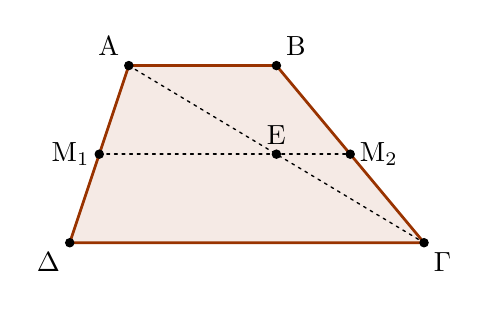
\begin{tikzpicture}[scale=.75]
\tkzSetUpLine[line width=1pt,color=black]
\tkzSetUpPoint[fill=black]

\tkzDefPoints{0/0/D,6/0/C,1/3/A,3.5/3/B}

\tkzDefMidPoint(A,D) \tkzGetPoint{M1}
\tkzDefMidPoint(B,C) \tkzGetPoint{M2}

\tkzDefPointBy[projection=onto C--D](A)\tkzGetPoint{H}

\tkzFillPolygon[fill=ShapeClr,fill opacity=0.1](A,B,C,D)

\tkzInterLL(A,C)(M1,M2) \tkzGetPoint{E}


\tkzDrawPolygon[color=ShapeClr](A,B,C,D)
\tkzDrawPoints[size=3](A,B,C,D,M1,M2,E)
\tkzLabelPoint[above left](A){$\rm A$}
\tkzLabelPoint[above right](B){$\rm B$}
\tkzLabelPoint[below right](C){$\rm \Gamma$}
\tkzLabelPoint[below left](D){$\rm \Delta$}
\tkzLabelPoint[above](E){$\rm E$}
\tkzLabelPoint[left](M1){$\rm M_1$}
\tkzLabelPoint[right](M2){$\rm M_2$}

\tkzDrawSegments[line width=0.5pt,color=black,dashed,dash pattern=on 1pt off 1.75pt](A,C M1,M2)

\end{tikzpicture}
\end{document}
